%!TEX root = skripsi.tex
%-----------------------------------------------------------------------------%
\chapter{\babDua}
%-----------------------------------------------------------------------------%
Bab ini membahas mengenai studi literatur yang digunakan selama penelitian. Studi literatur ini menjelaskan tentang hal-hal mendasar yang dibutuhkan dalam penelitian.
%-----------------------------------------------------------------------------%

\section{Lexical \textit{Semantic}}

Kata dalam suatu bahasa memiliki banyak fitur atau informasi yang terkandung di dalamnya. Informasi pada kata tersebut meliputi contoh-contoh seperti ortografi, POS Tag, dan juga makna kata. Informasi yang ada tersebut dapat dipergunakan sebagai fitur untuk merepresentasikan suatu kata.

\subsection{\textit{Word Feature}}
Ortografi meliputi permasalahan dalam suatu kata pada bahasa mengenai ejaan, kapitalisasi, pemenggalan kata, dan lain-lain. Pada bentuk kata (morfologi), Lemma merupakan bentuk kata "dasar" seperti misalnya "\textit{run}", \textit{"ran"}, dan "\textit{runs}" memiliki lemma yang sama yaitu "run". POS Tag atau Part of Speech Tag merupakan "kategori" dari suatu kata yang didefinisikan untuk membedakan kelas-kelas yang ada seperti misalnya \textit{proper noun} (nama orang, organisasi, nama tempat, dan lain-lain), \textit{verb} (kata kerja), \textit{adjective} (kata sifat seperti "marah", "senang", dan lain-lain), \textit{adverbial}, dan semacamnya. Makna kata menyimpan informasi dari arti sebuah kata, dan satu kata bisa memiliki lebih dari satu makna. Selain informasi dalam suatu kata, terdapat relasi antara satu kata dengan kata lain seperti misalnya sinonim, homonim, polisemi, dan lain-lain. Berdasarkan informasi pada \citep{sheeba2013unsupervised}, sinonim merupakan relasi pada kata-kata yang berbeda namun memiliki makna yang serupa, dan homonim merupakan kata dengan ejaan atau penulisan yang sama namun memiliki makna yang berbeda. Mirip dengan homonim, polisemi merupakan suatu kata yang memiliki makna lebih dari satu. Contoh dari relasi sinonim adalah antara kata "bohong" dengan "dusta", "perspektif" dengan "sudut pandang", dan kata-kata dengan makna mirip lainnya. Contoh dari kata polisemi adalah pada kata "darah" dalam kalimat "Tangan Ani mengeluarkan darah setelah tertusuk jarum" dengan "Ani baru menyadari bahwa dia dan Rina memiliki hubungan darah". Relasi homonim antar kata dapat dilihat misalnya pada kata "rapat" yang dapat berarti "pertemuan" ataupun juga "berdekatan", sebenarnya kata ini merupakan dua buah kata yang berbeda(sehingga maknanya berbeda) hanya saja penulisan dan pengejaannya sama.

Terdapat beberapa cara untuk merepresentasikan sebuah kata sebagai fitur. Salah satu cara yang sederhana adalah dengan merepresentasikan kata sebagai \textit{one hot vector}. Pada model ini, setiap kata di dalam sebuah korpus diberikan nomor indeks untuk membangun vektor yang mewakili keberadaan kata tersebut. Jika terdapat sebuah kata yang muncul pada konteks yang ingin direpresentasikan, indeks vektor yang sama dengan indeks kata tersebut akan bernilai 1. Bila terdapat sebuah korpus dengan jumlah kata unik berjumlah 4 dengan kata-kata "Ani", "marah", "kemarin", dan "malam" (sebuah vektor dengan pangjang empat). Representasi \textit{one hot vector} untuk kalimat "Ani marah" dapat ditulis dengan vektor [1,1,0,0].

Representasi \textit{one hot vector} akan mempunyai panjang vektor yang besar jika korpus mempunyai jumlah kata unik yang besar. Terdapat bentuk representasi lain untuk membentuk vektor dari kata, salah satunya adalah dengan \textit{word embedding}. \textit{Word Embedding} menggunakan representasi bilangan \textit{real} pada vektor untuk merepresentasikan sebuah kata berdasarkan hasil \textit{training} dengan suatu korpus. Contoh representasi dari \textit{word embedding} pada suatu kata "makan" adalah vektor [0.6, -0.3, ..., 0.5] (misalnya). Vektor dari hasil \textit{word embedding} mempunyai karakteristik dimana jarak antara dua buah vektor dari kata yang mirip secara semantik bernilai kecil(dekat). Bila misalkan pada data \textit{training} untuk \textit{word embedding} terdapat banyak kalimat-kalimat berbentuk "... makan Y ..." dimana Y adalah sebuah objek berupa makanan. Maka kata-kata yang mewakili Y seperti misalnya "burger", "apel", "steak", dan lain-lain, akan memiliki vektor yang mirip dan secara implisit dapat saling menggantikan untuk menempati posisi Y tersebut. Berdasarkan keterdekatan vektor tersebut, \textit{word embedding} mampu untuk menangkap semantik dari kata-kata yang ada pada korpus.

Salah satu model \textit{word embedding} yang dapat digunakan adalah Word2Vec \citep{mikolov2013distributed}. Pada penelitian ini Word2Vec akan digunakan untuk memanfaatkan vektor \textit{word embedding} sebagai salah satu fitur percobaan skenario yang ada. 

\subsection{Wordnet}

Wordnet merupakan \textit{online lexical database} yang didesain dan untuk digunakan suatu program \citep{miller1995wordnet}. Salah satu Wordnet untuk bahasa Inggris yang sudah berkembang dan digunakan dalam berbagai penelitian adalah Wordnet yang dikembangkan Princeton. Representasi yang digunakan Wordnet adalah \textit{set of synonyms} (synset) sebagai kumpulan dari kata-kata yang memiliki kemiripan makna. Selain menyimpan kata-kata, Wordnet juga menyimpan makna dari setiap kata-kata tersebut. Informasi makna kata yang ada di dalam Wordnet sering digunakan untuk sistem WSD suatu bahasa sebagai acuan (\textit{sense inventory}). Makna kata pada Wordnet disimpan dengan \textit{uniq identifier} berupa \textit{sense key} yang memiliki format "\textbf{lemma\%key}". Salah satu contoh \textit{sense key} adalah "home\%1:06:00::" yang mana memiliki makna "\textit{Housing that someone is living in}". Representasi \textit{synset} dari Wordnet beserta relasi-relasinya tersebut dapat dimanfaatkan untuk disambiguasi makna suatu kata.

%-----------------------------------------------------------------------------%
\section{Word Sense Disambiguation}
%-----------------------------------------------------------------------------%
\textit{Word Sense Disambiguation} merupakan salah satu penelitian di bidang NLP yang bertujuan untuk menentukan makna yang paling tepat dari suatu kata berdasarkan konteks kata tersebut ditemukan. Sebagaimana kata dalam suatu bahasa bisa memiliki makna lebih dari satu (polisemi), \textit{task} ini akan menentukan makna kata mana yang paling tepat. 

Penentuan makna kalimat dilakukan dengan pemberian informasi berupa kata yang menjadi \textit{target} dan konteks berupa kalimat. Contoh proses disambiguasi yang dilakukan untuk kata \textbf{cokelat}:

\begin{lstlisting}[backgroundcolor = \color{white}]
K1: Roni memakan cokelat yang diberikan ibunya
K2: Walaupun mobil cokelat itu mahal, dia sangat ingin membelinya
\end{lstlisting}


Pada kalimat pertama (K1), \textbf{cokelat} yang dimaksud memiliki makna sebagai makanan yang terbuat dari buah \textit{cokelat}. Sementara itu, Kata \textbf{cokelat} pada kalimat kedua (K2) memiliki makna yang berbeda, dimana kata tersebut merupakan satu keterangan warna. Penentuan makna yang tepat dapat dilakukan dengan bantuan informasi konteks dari kalimat dimana kata tersebut muncul. Pada K1, kata \textbf{memakan} memberikan informasi bahwa \textit{cokelat} yang dimaksud adalah objek yang bisa dimakan. Kata yang memberikan informasi pada kalimat kedua adalah kata \textbf{berwarna} yang secara eksplisit menerangkan bahwa \textbf{cokelat} yang dimaksud adalah warna. Namun demikian, konteks maupun informasi yang bisa diambil dari kalimat tidak selalu eksplisit. Pada contoh kalimat seperti "Pohon cokelat tua di belakang rumahku sangat besar", cokelat yang dimaksud bisa bermakna "buah cokelat yang sudah tua" atau "berwarna cokelat tua".

Penentuan makna kata yang tepat oleh sistem WSD ditentukan berdasarkan konteks dari kata tersebut berada. Walaupun satu kata dapat memiliki beberapa makna, terdapat kecil kemungkinan bahwa kata yang sama digunakan dalam satu \textit{discourse} (konten dari sebuah percakapan atau bahasan) untuk menyatakan makna yang berbeda sebagaimana "\textit{one sense per discourse}" \citep{gale1992one}.

Pada umumnya, sistem WSD yang dibangun dapat menggunakan pendekatan \textit{machine learning} baik itu \textit{supervised}, \textit{semi-supervised}, maupun \textit{unsupervised}. Pendekatan yang dipilih biasanya bergantung pada data maupun \textit{resource} yang dimiliki pada suatu bahasa. Jika terdapat data/\textit{resource} yang memadai, sistem dengan pendekatan \textit{supervised} biasanya dilakukan untuk mendapatkan akurasi yang optimal. Namun demikian, untuk bahasa-bahasa dengan data/\textit{resource} yang kurang memadai, pendekatan \textit{semi-supervised} atau bahkan \textit{unsupervised} dapat dimanfaatkan untuk mendapatkan makna kata secara otomatis. Terdapat dua buah granularitas dalam sistem WSD yaitu \textit{coarse-grain} dan \textit{fine-grain}. Perbedaan utama yang membedakan adalah \textit{fine-grain} memiliki \textit{sense inventory} yang lebih detail dan dengan kemiripan makna antar kata yang lebih rinci dibandingkan dengan \textit{coarse-grain}. Pada sistem WSD, fitur yang umum digunakan beberapa diantaranya adalah konteks kata baik dengan pendekatan Collocation dan Co-occurrence, POS Tag kata, vektor \textit{word embedding} kata. Fitur Co-occurrence lebih berfokus pada kemunculan kata pada suatu konteks baik itu dokumen, paragraf, atau kalimat, sementara Collocation lebih berfokus pada kata yang sering muncul secara bersama-sama dan kecil kemungkinannya untuk muncul bersama secara kebetulan. 

\subsection{WSD Bahasa Inggris Menggunakan IMS \textit{Disambiguation System}}
Salah satu sistem WSD untuk bahasa inggris yang ada adalah "It Makes Sense" (IMS) yang dibuat oleh Zhi Zhong dan Hwee Tou Ng \citep{zhong2010makes}. Sistem  dibangun menggunakan pendekatan \textit{supervised learning} yang dapat digunakan untuk semua kata bahasa Inggris. Pada dasarnya, \textit{classifier} yang dipilih untuk \textit{task} ini adalah \textit{support vector machine} (SVM). Arsitektur yang dibangun pada IMS dapat dilihat pada gambar berikut:

\begin{figure}
	\centering
	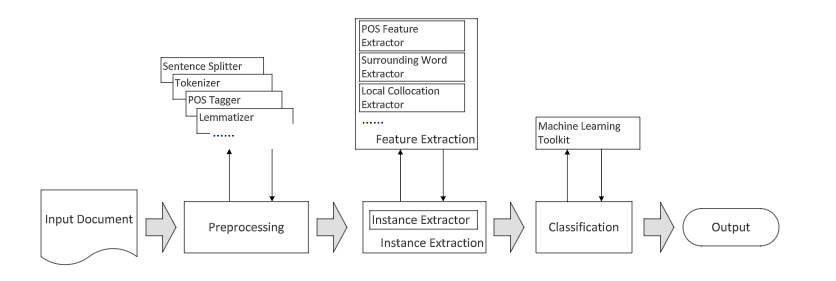
\includegraphics[width=1\linewidth]{adit_pics/Arsitektur-IMS}
	\caption{Arsitektur IMS}
	\label{fig:Arsitektur-IMS}
\end{figure}

Proses \textit{pre-processing} pada IMS dilakukan dengan empat tahapan:
\begin{enumerate}
	\item Mendeteksi batasan kalimat dengan \textit{sentence splitter}
	\item Tokenisasi dengan \textit{tokenizer}
	\item POS Tagging untuk semua token
	\item Mengubah token menjadi lemma dengan \textit{lemmatizer}
\end{enumerate}

Ekstraksi fitur dilakukan dengan mengombinasikan:

\begin{enumerate}
	\item POS Tag dari tiga buah kata di kiri dan kanan \textit{target word}, serta kata itu sendiri. 
	\item Kata-kata sekitar pada konteks kalimat ataupun kalimat tetangganya. Kata-kata yang terkandung di dalam \textit{stopwords} dan memiliki simbol atau angka dibuang dari kalimat tersebut. Kata-kata yang tersisa tersebut kemudian diubah menjadi bentuk kata dasarnya dalam huruf kecil.
	\item \textit{Local Collocation} dengan 11 buah \textit{collocation} baik itu sebelum \textit{target word} maupun setelahnya. 
\end{enumerate}

Pengujian seberapa baik performa IMS dalam melakukan  WSD \textit{task} mendapatkan hasil:

\begin{figure}
	\centering
	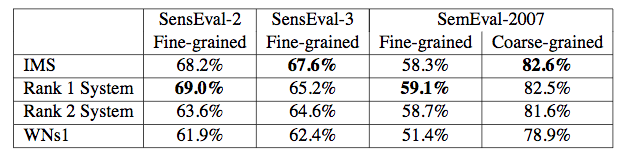
\includegraphics[width=1\linewidth]{adit_pics/Performa-IMS}
	\caption{Performa IMS \citep{zhong2010makes}}
	\label{fig:Performa-IMS}
\end{figure}

IMS digunakan pada penelitian ini karena sistem WSD ini sudah dapat digunakan untuk \textit{tagging} makna kata dengan input berupa \textit{free text}.

%-----------------------------------------------------------------------------%
\section{Word Sense Induction}
%-----------------------------------------------------------------------------%	
%-----------------------------------------------------------------------------%	
\textit{Word Sense Induction} (WSI) adalah sebuah \textit{task} yang mempunyai fungsi utama untuk mendapatkan makna kata dari sebuah korpus atau teks yang belum dianotasi secara otomatis. WSI dapat dilakukan jika penelitian WSD yang ingin dilakukan tidak mempunyai cukup \textit{resource} seperti misalnya Wordnet ataupun \textit{sense tagged corpus} yang memadai. WSI secara tidak langsung dapat memperbanyak data yang dapat digunakan jika sistem WSD yang ingin dibangun membutuhkan data \textit{training} yang tidak sedikit. Terdapat berbagai macam pendekatan dalam melakukan \textit{sense induction}, diantaranya adalah dengan melakukan \textit{clustering} kata \citep{denkowski2009survey}, ataupun menggunakan pendekatan \textit{cross language}.
	
	\subsection{Pendekatan \textit{Clustering}}
	Dua kata dianggap dekat secara semantik jika memiliki \textit{co-occurrence} dengan kata-kata tetangganya yang sama \citep{nasiruddin2013state}. Konsep tersebut mendasari cara WSI mendapatkan \textit{sense} kata secara implisit berdasarkan hasil \textit{cluster} yang terbentuk dari data atau teks mentah (teks yang tidak dianotasi).
	
	Penarikan makna secara implisit dapat dicontohkan pada beberapa kalimat rujukan berikut \citep{denkowski2009survey}:
	
	\begin{enumerate}
		\item A bottle of tezg\"{u}no is on the table.
		\item Everyone likes tezg\"{u}no.
		\item Tezg\"{u}no makes you drunk.
		\item We make tezg\"{u}no out of corn.
	\end{enumerate}
	
	Walaupun belum terdapat informasi eksplisit makna dari tezg\"{u}no, dapat disimpulkan bahwa tezg\"{u}no mengacu pada minuman beralkohol yang memabukkan. Penarikan kesimpulan ini didapatkan dari kemunculan kata tersebut dengan kata lain pada konteks yang sama.
	
	Pada pendekatan \textit{clustering} ini, makna kata bisa didapatkan secara implisit dari hasil \textit{cluster} yang terbentuk, namun demikian pelabelan yang dilakukan untuk menentukan apa yang direpresentasikan \textit{cluster} tersebut merupakan sebuah \textit{task} tersendiri.
	
	Salah satu cara \textit{clustering} yang dijelaskan pada \citep{pantel2002discovering} adalah dengan mencoba beberapa algoritma seperti K-Means, Buckshot, CBC, Unicon, Bisecting K-Means, dan Average Link untuk fitur yang ditentukan. Fitur yang digunakan adalah vektor dari kata yang didapatkan dengan menghitung \textit{discounted pointwise mutual information} dari kata tersebut pada konteks kata itu muncul. Perhitungan \textit{similarity} antara dua buah kata dihitung dengan menghitung jarak vektor kedua kata tersebtu.
	
	\subsection{Pendekatan \textit{Cross Language}}
	Selain pendekatan \textit{clustering}, WSI juga dapat memanfaatkan fitur dimana satu kata dari suatu bahasa, dapat diterjemahkan menjadi beberapa kata di bahasa lain. Contoh kasus tersebut dapat dilihat pada kata "halaman" berikut:

	\begin{lstlisting}[backgroundcolor = \color{white}]
	(K1-Indonesia): Aku membaca 10 halaman buku Harry Potter
	(K1-English): I read 10 pages of Harry Potter book
	(K2-Indonesia): Ani tinggal di rumah dengan halaman yang sangat luas
	(K2-English): Ani lives in a house with very large yard
	\end{lstlisting}
	
	Berdasarkan kedua pasangan kalimat tersebut, kata \textbf{halaman} dalam bahasa Indonesia dapat diterjemahkan menjadi dua buah kata dalam bahasa Inggris, yaitu \textit{page} ataupun \textit{yard}. Hal ini menunjukan bahwa terjemahan dari suatu kata bergantung pada konteks dimana kata tersebut muncul.
	
	Salah satu penelitian yang juga menggunakan pendekatan \textit{Cross-Lingual} WSI adalah penelitian \citep{septiantri2013wsd} yang memanfaatkan korpus paralel untuk menentukan makna yang tepat dari suatu kata berdasarkan makna tersebut dalam Bahasa Indonesia dan Bahasa Inggris.


\section{Korpus Paralel dan \textit{Comparable}}
Terdapat dua macam korpus bilingual yang dapat dimanfaatkan untuk pemanfaatan \textit{cross language } WSD yaitu korpus paralel dan \textit{comparable}. Perbedaan utama terhadap kedua buah korpus berada pada seberapa identik kedua buah konteks yang dimilikinya. Korpus paralel memiliki kalimat dan kata-kata yang serupa antara dua buah pasangan di masing-masing korpus. Hal ini dapat dicontohkan misalnya dengan kalimat satu pada korpus bahasa Indonesia "Aku makan" dengan "I eat" pada korpus bahasa Inggris. Berbeda dengan korpus paralel, \textit{comparable} berarti kedua kalimat atau \textit{instance} yang berpasangan hanya sebatas mirip/sama dalam suatu kategori kriteria tertentu. Dengan adanya korpus paralel dan \textit{comparable} tersebut, dibutuhkan juga alat untuk menyelaraskan (\textit{aligning}) konten pada kedua korpus tersebut. \textit{Alignment} yang dapat dilakukan memiliki beberapa tingkatan mulai dari \textit{scope} yang besar sampai kecil. \textit{Scope} besar tersebut meliputi \textit{alignment} dokumen yang mana fungsinya adalah menyelaraskan antar dokumen yang konten atau kriterianya sama. Tingkatan yang lebih kecil berikutnya yaitu kalimat dimana \textit{alignment} dilakukan pada \textit{level} kalimat (pasangan kalimat yang makna atau kriterianya sama). \textit{Alignment} dengan tingkatan yang lebih spesifik lagi adalah kata (\textit{word alignment}), dimana hasil yang didapat dari proses ini adalah pasangan kata pada kedua korpus dwibahasa yang selaras. Korpus utama yang digunakan sebagai sumber data penelitian ini adalah korpus identik \citep{larasati2012identic}. Korpus identik berisi pasangan kalimat-kalimat dalam bahasa Indonesia dan Inggris. Kalimat yang berpasangan di dalamnya sebagian besar mempunyai makna konten yang paralel walaupun terdapat juga yang \textit{comparable}. Korpus identik ini mempunyai total sebanyak 88.918 buah pasangan kalimat di dalamnya. Format korpus identik adalah sebagai berikut:
\begin{lstlisting}
<ID><tab><Kalimat Indonesia><tab><Kalimat Inggris>
\end{lstlisting}
Contoh isi dari korpus identik yang digunakan berbentuk seperti berikut ini:
\begin{lstlisting}[backgroundcolor = \color{white}]
...
panl-bppt-eco-s1505	Ada 10 sektor yang dibicarakan.	There are 10 sectors that have been on the talk.
panl-bppt-eco-s1508	Semua ketentuan Insya Allah akan selesai 1 April, kata Burhanuddin.	All the regulations, God willing, will be completed on April 1, he said.
...
\end{lstlisting}

%-----------------------------------------------------------------------------%
\section{\textit{Word Alignment}}
Tugas dari \textit{word alignment} adalah menemukan korespondensi antara kata pada teks paralel 
\citep{mihalcea2003evaluation}. Secara umum, proses dari pemasangan kata berlangsung seperti pada gambar \ref{fig:word-alignment}.


\begin{figure}
	\centering
	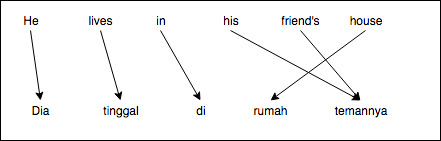
\includegraphics[width=1\linewidth]{adit_pics/wordalignment.jpeg}
	\caption{Word Alignment}
	\label{fig:word-alignment}
\end{figure}

Kasus yang dapat terjadi pada proses \textit{alignment} ini salah satunya adalah ketika terdapat kata yang tidak memiliki pasangan. Contoh dari kasus tersebut dapat dilihat pada pasangan kalimat berikut:

\begin{lstlisting}[backgroundcolor = \color{white}]
K1(en) : He would do it regardless what people say
K1(id) : Dia akan melakukannya segalanya
\end{lstlisting}


Bila melihat bahasa Indonesia sebagai sumber bahasa, maka kata "segalanya" pada kalimat tersebut tidak memiliki pasangan dalam bahasa Inggris K1. Pada kasus-kasus seperti ini, biasanya akan ada token khusus yang nantinya akan berpasangan dengan kata-kata yang tidak mempunyai pasangan.

Selain kata yang tidak memiliki pasangan, terdapat juga kasus dimana pasangan adalah berupa frasa. Hal ini dapat dilihat pada contoh berikut:

\begin{lstlisting}[backgroundcolor = \color{white}]
K2(en) : The victim must be taken to the hospital
K2(id) : Korban tersebut harus di bawa ke rumah sakit
\end{lstlisting}

Pada contoh pasangan kalimat tersebut, kata "\textit{hospital}" berpasangan dengan "rumah sakit". Proses pemasangan kata dengan frasa lebih sulit dibandingkan dengan satu unit kata saja.

\textit{Tool} yang digunakan untuk keperluan \textit{word alignment} pada penelitian ini adalah Giza++ \citep{och03:asc}. \textit{Tool} tersebut merupakan salah satu \textit{word alignment tools} pada \textit{statistical machine translation} (SMT) yang dapat digunakan untuk memasangkan kata-kata pada dua buah korpus dwibahasa atau lebih. Terdapat beberapa \textit{word alignment tools} lain seperti Berkeley \textit{aligner}, anymalign, dan lain-lain.
%------------------------------------------- ----------------------------------%

\section{Support Vector Machine}
Salah satu \textit{classifier} yang dapat digunakan dalam \textit{supervised learning} untuk melakukan klasifikasi adalah SVM. SVM termasuk sebagai metode klasifikasi yang populer dan telah digunakan untuk berbagai permasalahan seperti klasifikasi teks, \textit{facial expression recognition}, analisis gen, \textit{word sense disambiguation}, dan lain-lain. SVM dapat dikatakan sebagai salah satu metode yang membangun aturan yang dinamakan sebagai \textit{linear classifier} yang secara teori akan menghasilkan kualitas prediksi dari \textit{unseen data} yang baik \citep{fradkin2006support}. Pada salah satu penelitian WSD Bahasa Inggris \citep{zhong2010makes}, SVM digunakan sebagai \textit{classifier} dari sistem yang dibuat.

Konsep dari cara SVM bekerja adalah dengan menemukan sebuah \textit{hyperplane} dengan \textit{margin} (jarak dari \textit{hyperplane} dengan titik kelas terdekat) yang terbesar. Pemilihan \textit{margin} dengan nilai terbesar ini ditujukan agar \textit{classifier} lebih optimal dalam memisahkan objek dengan kelas yang berbeda. Pada penelitian kali ini, SVM yang digunakan berasal dari \textit{library} Python bernama Scikit \citep{scikit-learn}.

\section{Evaluasi}

Precision, Recall, dan F-score merupakan beberapa cara perhitungan untuk merepresentasikan akurasi dari suatu sistem. Berdasarkan domain \textit{information retrieval}, precision merupakan perbandingan dari total jumlah dokumen relevan yang didapatkan oleh sistem dengan total jumlah dokumen yang didapat. Lain halnya dengan precision, recall membandingkan total dokumen relevan yang didapatkan dengan total dokumen relevan dalam \textit{database} \citep{ting2011precision}. Kedua penilaian ini juga digunakan pada sistem yang melakukan klasifikasi suatu \textit{instance} dengan kelas-kelas yang sudah ditentukan.

Pada kasus \textit{word alignment}, terdapat empat buah pengukuran yang dapat dilakukan yaitu \textit{precision}, \textit{recall}, \textit{f-measure}, dan \textit{alignment error rate (AER)} \citep{mihalcea2003evaluation}. Diberikan hasil \textit{alignment} dari program berupa A, dan \textit{gold standard alignment} dari \textit{evaluator} (manusia) sebagai G, masing-masing mengandung dua buah \textit{set} yaitu \textit{probable alignment} dan \textit{sure alignment}. Karena \textit{tool alignment} yang digunakan pada penelitian ini menghasilkan \textit{sure alignment} untuk setiap pasangan, maka dilakukan penyesuaian formula penghitungan seperti rumus pada (2.1).

\begin{equation}
\begin{split}
Precision = A \cap G / A \\
Recall = A \cap G / G \\
FScore = 2 P R / P + R
\end{split}
\end{equation}

Dikarenakan proses \textit{word alignment} pada penelitian ini tidak membedakan antara \textit{probable} dan \textit{sure alignment}, maka semua hasil \textit{alignment} dianggap merupakan set dari \textit{sure alignment}.

Evaluasi yang dilakukan pada sistem WSD yang dibuat juga menggunakan nilai precision dan recall untuk menghitung F-Score. Pada perhitungan F-Score tersebut, teknik \textit{cross validation} juga digunakan untuk membagi data menjadi \textit{training} dan \textit{testing set} dan hasil perhitungan F-Score nantinya akan diambil rata-ratanya dari setiap \textit{fold} \textit{cross validation}.